\begin{figure}[!h]
\centering
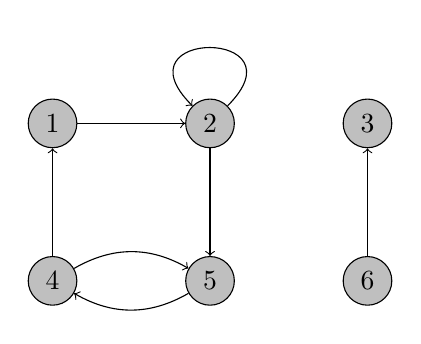
\begin{tikzpicture}[scale=1, vertex/.style = {circle,fill=gray!50,draw}, edge/.style = {->,thin}]
% vertex
\node[vertex] (n4) at (1,1) {4};
\node[vertex] (n5) at (3,1) {5};
\node[vertex] (n2) at (3,3) {2};
\node[vertex] (n1) at (1,3) {1};
\node[vertex] (n6) at (5,1) {6};
\node[vertex] (n3) at (5,3) {3};
%edges
\draw[edge] (n4) to (n1);
\draw[edge] (n1) to (n2);
\draw[edge] (n2) to (n5);
\draw[edge] (n6) to (n3);
\draw[edge] (n4) to[bend left] (n5);
\draw[edge] (n5) to[bend left] (n4);
\draw[edge] (n2) to[loop] (n2);
\end{tikzpicture}
\caption{Grafo direccionado}
Un grafo direccionado $G=(V,E)$, donde $V=\{1,2,3,4,5,6\}$ y $E=\{(1,2),(2,2),(2,4),(2,5),(4,1),(4,5),(4,5),(6,3)\}$. \\Fuente: \cite{Cormen2009}.
\label{grafoDir}
\end{figure}